\starredchapter{ANNEXE~\thechapter. ESTIMATION DE LA TAILLE DES RESTES DE PROIES}\label{app:size-at-age}

Nous avons combiné les estimations de l'incertitude d'assignation de l'âge et la taille selon l'âge spécifique au stock pour convertir les estimations de l'âge marin des restes de proies des ERSN en estimations de la probabilité qu'un échantillon donné appartienne à une des quatre classes de taille.

\appsection{Incertitude d'assignation de l'âge}

Les restes de proies des ERSN ont été âgés en utilisant les annuli d'écailles par des techniciens du laboratoire de détermination de l'âge des poissons au laboratoire de sclérochronologie de la station biologique du Pacifique (Pêches et Océans Canada, Nanaimo, Colombie-Britannique, Canada). Les assignations d'âge basées sur les écailles sont couramment utilisées dans les évaluations de stock de saumon du Pacifique et l'exactitude est typiquement élevée \citep{mcnicolAccuracyUsingScales2010}; cependant, ces estimations peuvent dévier de l'âge véritable résultant en erreur. Nous avons d'abord estimé l'ampleur et la direction (c.-à-d., surestimation vs. sous-estimation) de l'erreur de détermination de l'âge en utilisant des données de saumon chinook avec à la fois un âge estimé à partir des lectures d'écailles, ainsi qu'un âge connu des étiquettes de fil codé ou des étiquettes basées sur la parenté. Nous avons ensuite ajusté un modèle hiérarchique pour estimer l'erreur de détermination de l'âge associée à un échantillon collecté à partir des restes de proies des ERSN.

Les données d'âge estimé et véritable étaient disponibles pour 16 528 saumons chinook. Ces données provenaient du jeu de données de la pêche récréative présenté dans le texte principal, ainsi que des données de l'Évaluation des stocks du Fraser et de l'intérieur, qui ont collecté des échantillons dans le cadre de pêches d'essai en eau douce et d'échantillonnage d'échappée. Bien que des échantillons étaient disponibles pour chacun des stocks inclus dans le texte principal, les tailles d'échantillon spécifiques au stock variaient largement (p. ex., deux échantillons pour Columbia River Spring, 4 508 pour Fraser River Fall). Nous n'avons pas tenu compte de l'incertitude d'assignation du stock dans cette analyse. Chaque échantillon a été assigné à une des trois catégories de biais : zéro (âges estimé et véritable étaient identiques), sous-estimation (âge véritable supérieur à l'âge estimé), ou surestimation (âge véritable inférieur à l'âge estimé). Nous avons exclu 48 échantillons où la différence entre les âges véritables et estimés était supérieure à une année. 

La directionalité des erreurs différait entre les âges estimés -- les poissons estimés être plus âgés que quatre ans étaient plus susceptibles d'être surestimés, tandis que ceux estimés être plus jeunes que quatre ans étaient plus susceptibles d'être sous-estimés (Figure \ref{fig:age-error-bar}). L'exactitude était aussi typiquement la plus élevée pour les classes d'âge dominantes dans un stock (Figure \ref{fig:age-error-bar}).

\begin{figure}[htb]
    \centering
    \pdftooltip{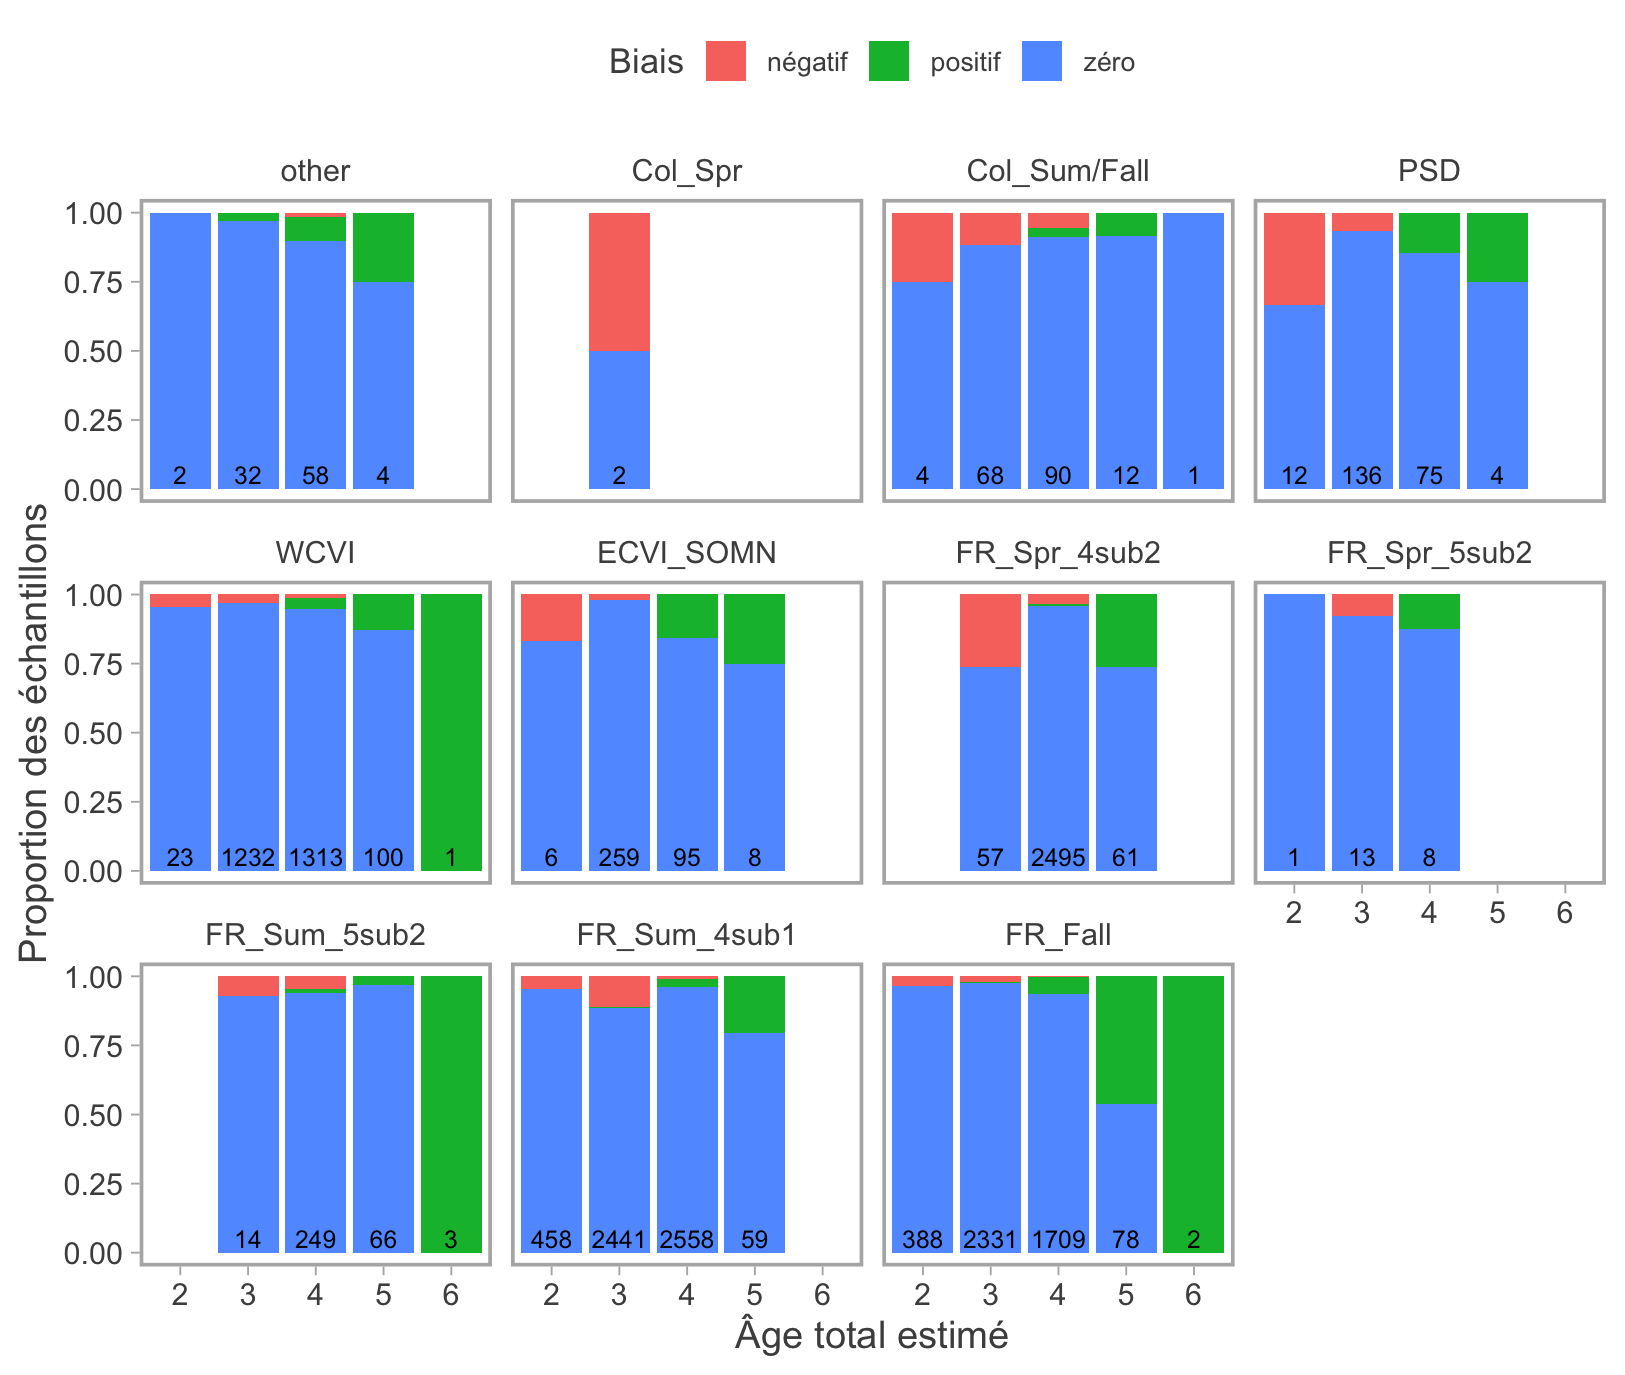
\includegraphics[width=5in]{figs/supp_figs/age_error.png}}{Figure \ref{fig:age-error-bar}}
    \caption{Biais dans l'âge total estimé parmi les stocks de saumon chinook. Les chiffres représentent le nombre d'échantillons dans une classe d'âge et un stock donnés.}
    \label{fig:age-error-bar}
\end{figure}

Pour générer des estimations d'erreur de détermination de l'âge pour les restes de proies des ERSN, nous avons ajusté un modèle multinomial hiérarchique dans lequel les trois catégories de biais (zéro, sous, ou sur) étaient la variable réponse, l'âge estimé était un effet fixe, et l'identité du stock était une interception aléatoire. Cette structure nous a permis de générer des taux d'erreur spécifiques à l'âge et au stock, tout en exploitant les stocks riches en données pour informer les stocks limités en données. Nous avons ajusté le modèle dans Stan via le paquet brms \citep{burknerBrmsPackageBayesian2017}, en utilisant des a priori faiblement informatifs. Nous avons utilisé le modèle ajusté pour convertir l'âge estimé associé à chaque échantillon de proie des ERSN en un vecteur de probabilités d'assignation de l'âge total $a_t$ $\boldsymbol{q_{a_t}}$, qui incorporait les taux d'erreur spécifiques à l'âge et au stock. Par exemple, un échantillon identifié comme provenant d'un individu Fraser Fall avec un âge total estimé de cinq ans pourrait résulter en une probabilité de 50\,\% d'être âgé de 4 ans et une probabilité de 50\,\% d'être âgé de 5 ans. 

\appsection{Estimations de taille selon l'âge}

Pour estimer la taille des proies à partir d'échantillons d'écailles, nous avons utilisé un modèle statistique pour prédire la taille selon l'âge en utilisant des données de la pêche récréative de saumon chinook. Ici, nous avons supposé qu'une probabilité d'assignation de stock supérieure à 75\,\% était exacte et avons exclu les échantillons en dessous de ce seuil. Les estimations d'âge marin, de taille corporelle et d'identité de stock étaient disponibles pour 7 815 saumons chinook plus grands que 550 mm de longueur à la fourche. Nous avons estimé la taille $b$ pour le stock $s$ en utilisant le modèle additif généralisé suivant :

\begin{align}
\label{eq:size_eq}
\tag{1}
b_{s} &\sim \operatorname{Normal} \left( \mu_{b_s}, \sigma^2 \right),\\
\tag{2}
\mu_{b_s} &= \alpha_s + \alpha_a + f_{w}w + f_{w_{s}}w + f_{w_{a}}w + \alpha_y \\
\notag
\end{align}
\noindent

Où $\alpha_a$ représente une interception pour l'âge marin $a$ et $\alpha_s$ représente une interception pour chaque stock. Nous avons représenté les changements saisonniers de taille corporelle avec $f_{w}$, une fonction lisse de processus gaussien pour la semaine d'échantillonnage $w$. Nous avons aussi permis à la variabilité saisonnière de différer entre les stocks et les classes d'âge marin, en utilisant des lissages hiérarchiques $f_{w_s}$ et $f_{w_a}$. Finalement, nous avons inclus une interception aléatoire $\alpha_y$ représentant les changements spécifiques à l'année dans la taille moyenne. Nous avons modélisé $\alpha_y$ en supposant une hyperdistribution avec une moyenne zéro et un écart-type $\sigma_y$. Notez que les groupements de stocks utilisés dans le modèle de taille selon l'âge étaient plus finement résolus que ceux utilisés dans les analyses de composition de stock pour augmenter la précision des prédictions.

Nous avons utilisé le modèle ajusté pour visualiser les motifs saisonniers dans la taille selon l'âge spécifique au stock et prédire la taille moyenne de chaque échantillon de proie des ERSN qui avait une estimation d'âge viable basée sur l'identité du stock associé et la semaine d'échantillonnage. Nous n'avons pas généré de prédictions spécifiques à l'année (c.-à-d., intégré hors $\alpha_y$) étant donné que de nombreux échantillons ont été collectés avant l'échantillonnage de la pêche récréative. 

Les stocks de saumon chinook capturés dans la zone d'étude différaient en âge marin, mais généralement les individus d'âge marin 2 et 3 étaient les plus communs (Figure \ref{fig:rec-age-comp}). Notez que ces observations sous-représenteront les individus d'âge marin 1 et 2 (particulièrement pour les histoires de vie de juvéniles de l'année) parce qu'ils excluent les individus plus petits que 550 mm de longueur à la fourche pour rester cohérent avec le reste de l'analyse.

\begin{figure}[htb]
    \centering
    \pdftooltip{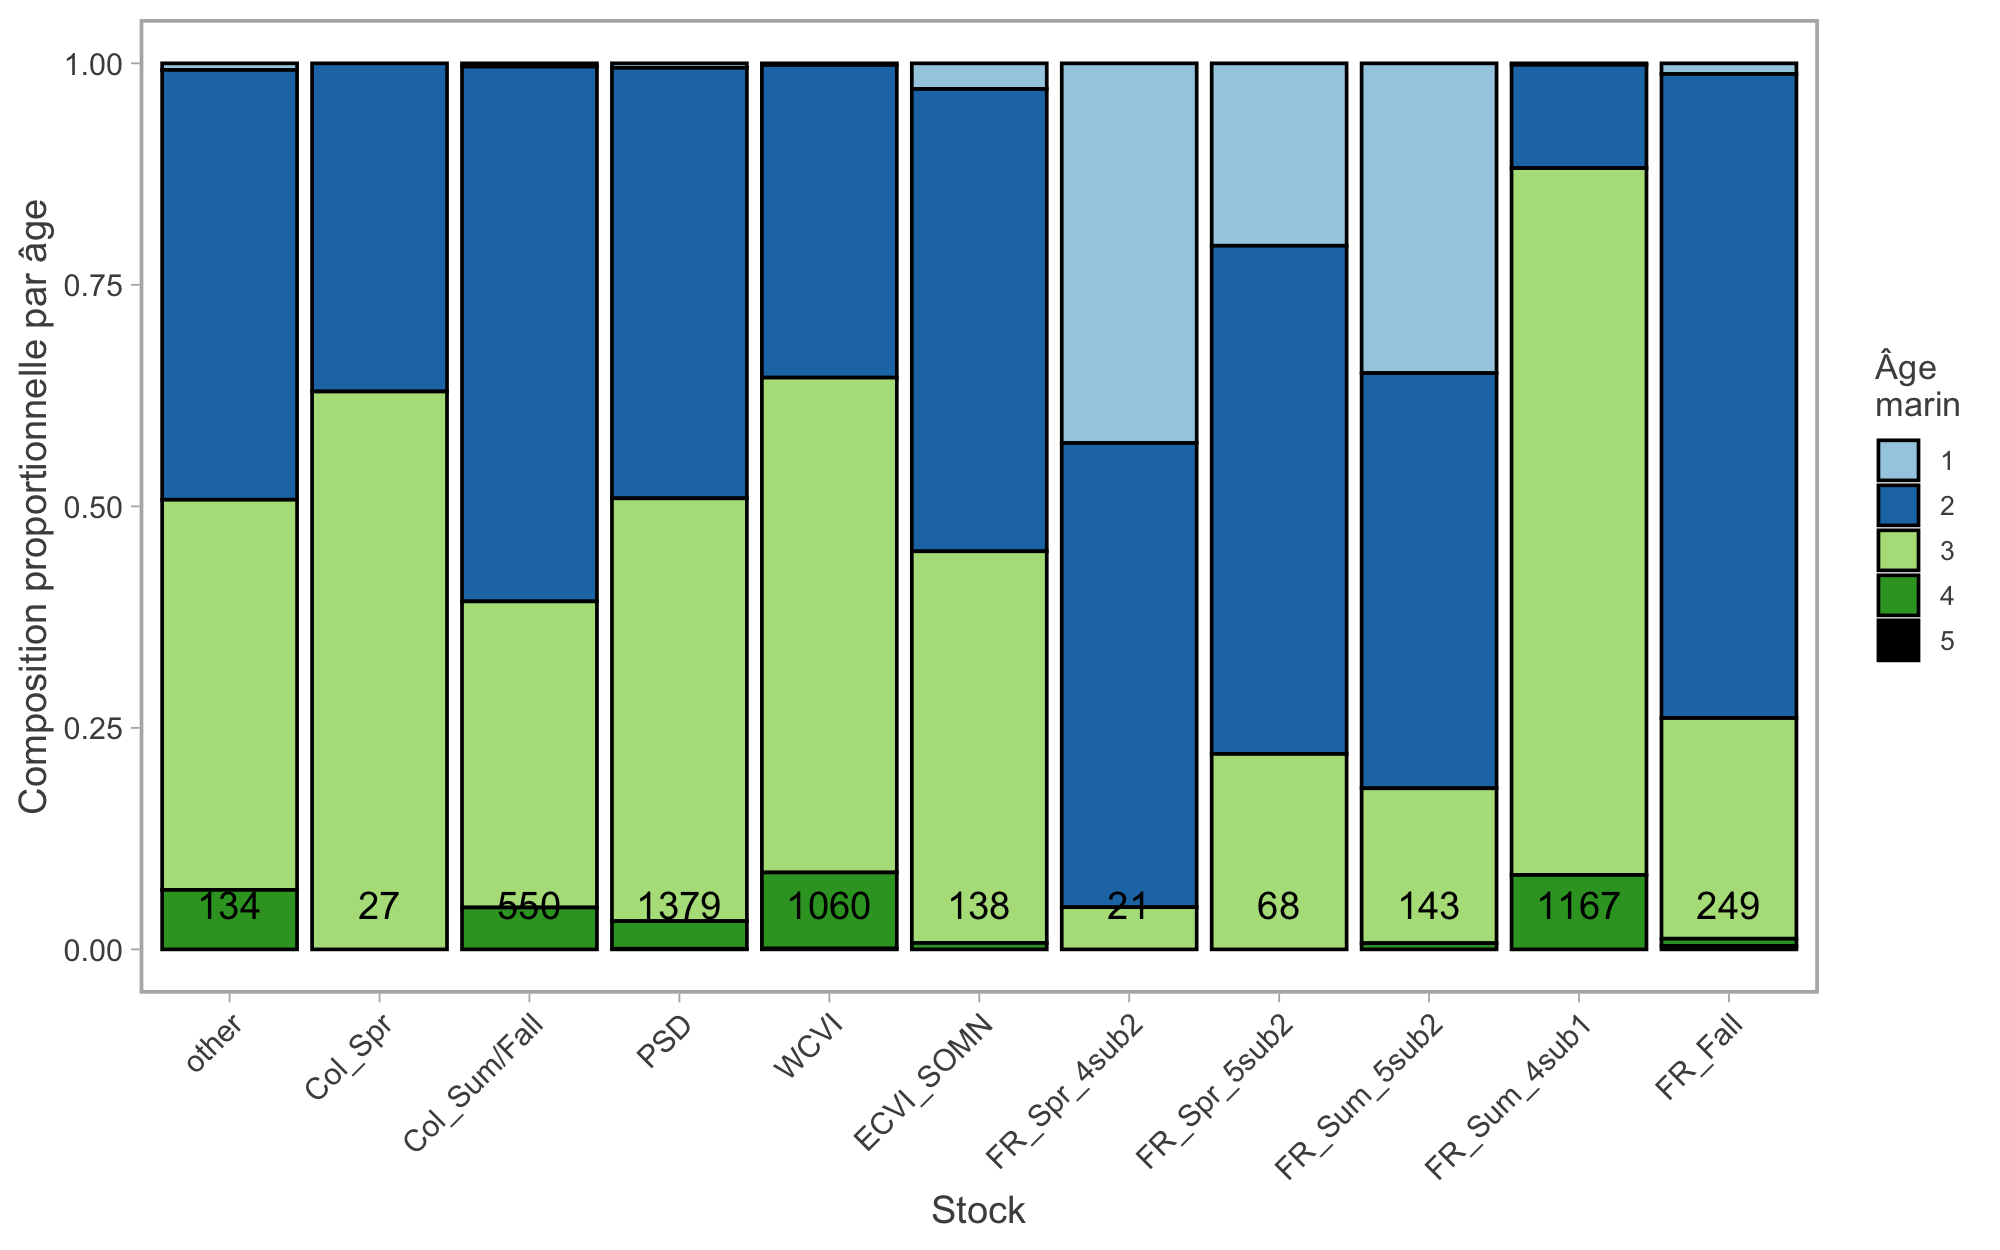
\includegraphics[width=5in]{figs/supp_figs/comp_bar_fishery_age_sw.png}}{Figure \ref{fig:rec-age-comp}}
    \caption{Âge marin observé du saumon chinook des pêches récréatives du sud de la C.-B.}
    \label{fig:rec-age-comp}
\end{figure}

Les âges marins plus vieux étaient plus grands que les âges marins plus jeunes et les stocks variaient en taille selon l'âge, avec les stocks de juvéniles d'un an typiquement plus grands à l'âge marin 2 que les stocks de juvéniles de l'année (Figure \ref{fig:pred-size-at-age}). Le saumon chinook a montré des preuves de changements dans la taille corporelle au cours de l'été; cependant, ces tendances différaient entre les stocks et entre les classes d'âge marin. Le modèle a capturé avec précision la variabilité de taille à l'intérieur des classes d'âge, ce qui a résulté en des distributions de taille qui se chevauchent (Figure \ref{fig:hist-size-at-age}). 

\begin{figure}[htb]
    \centering
    \pdftooltip{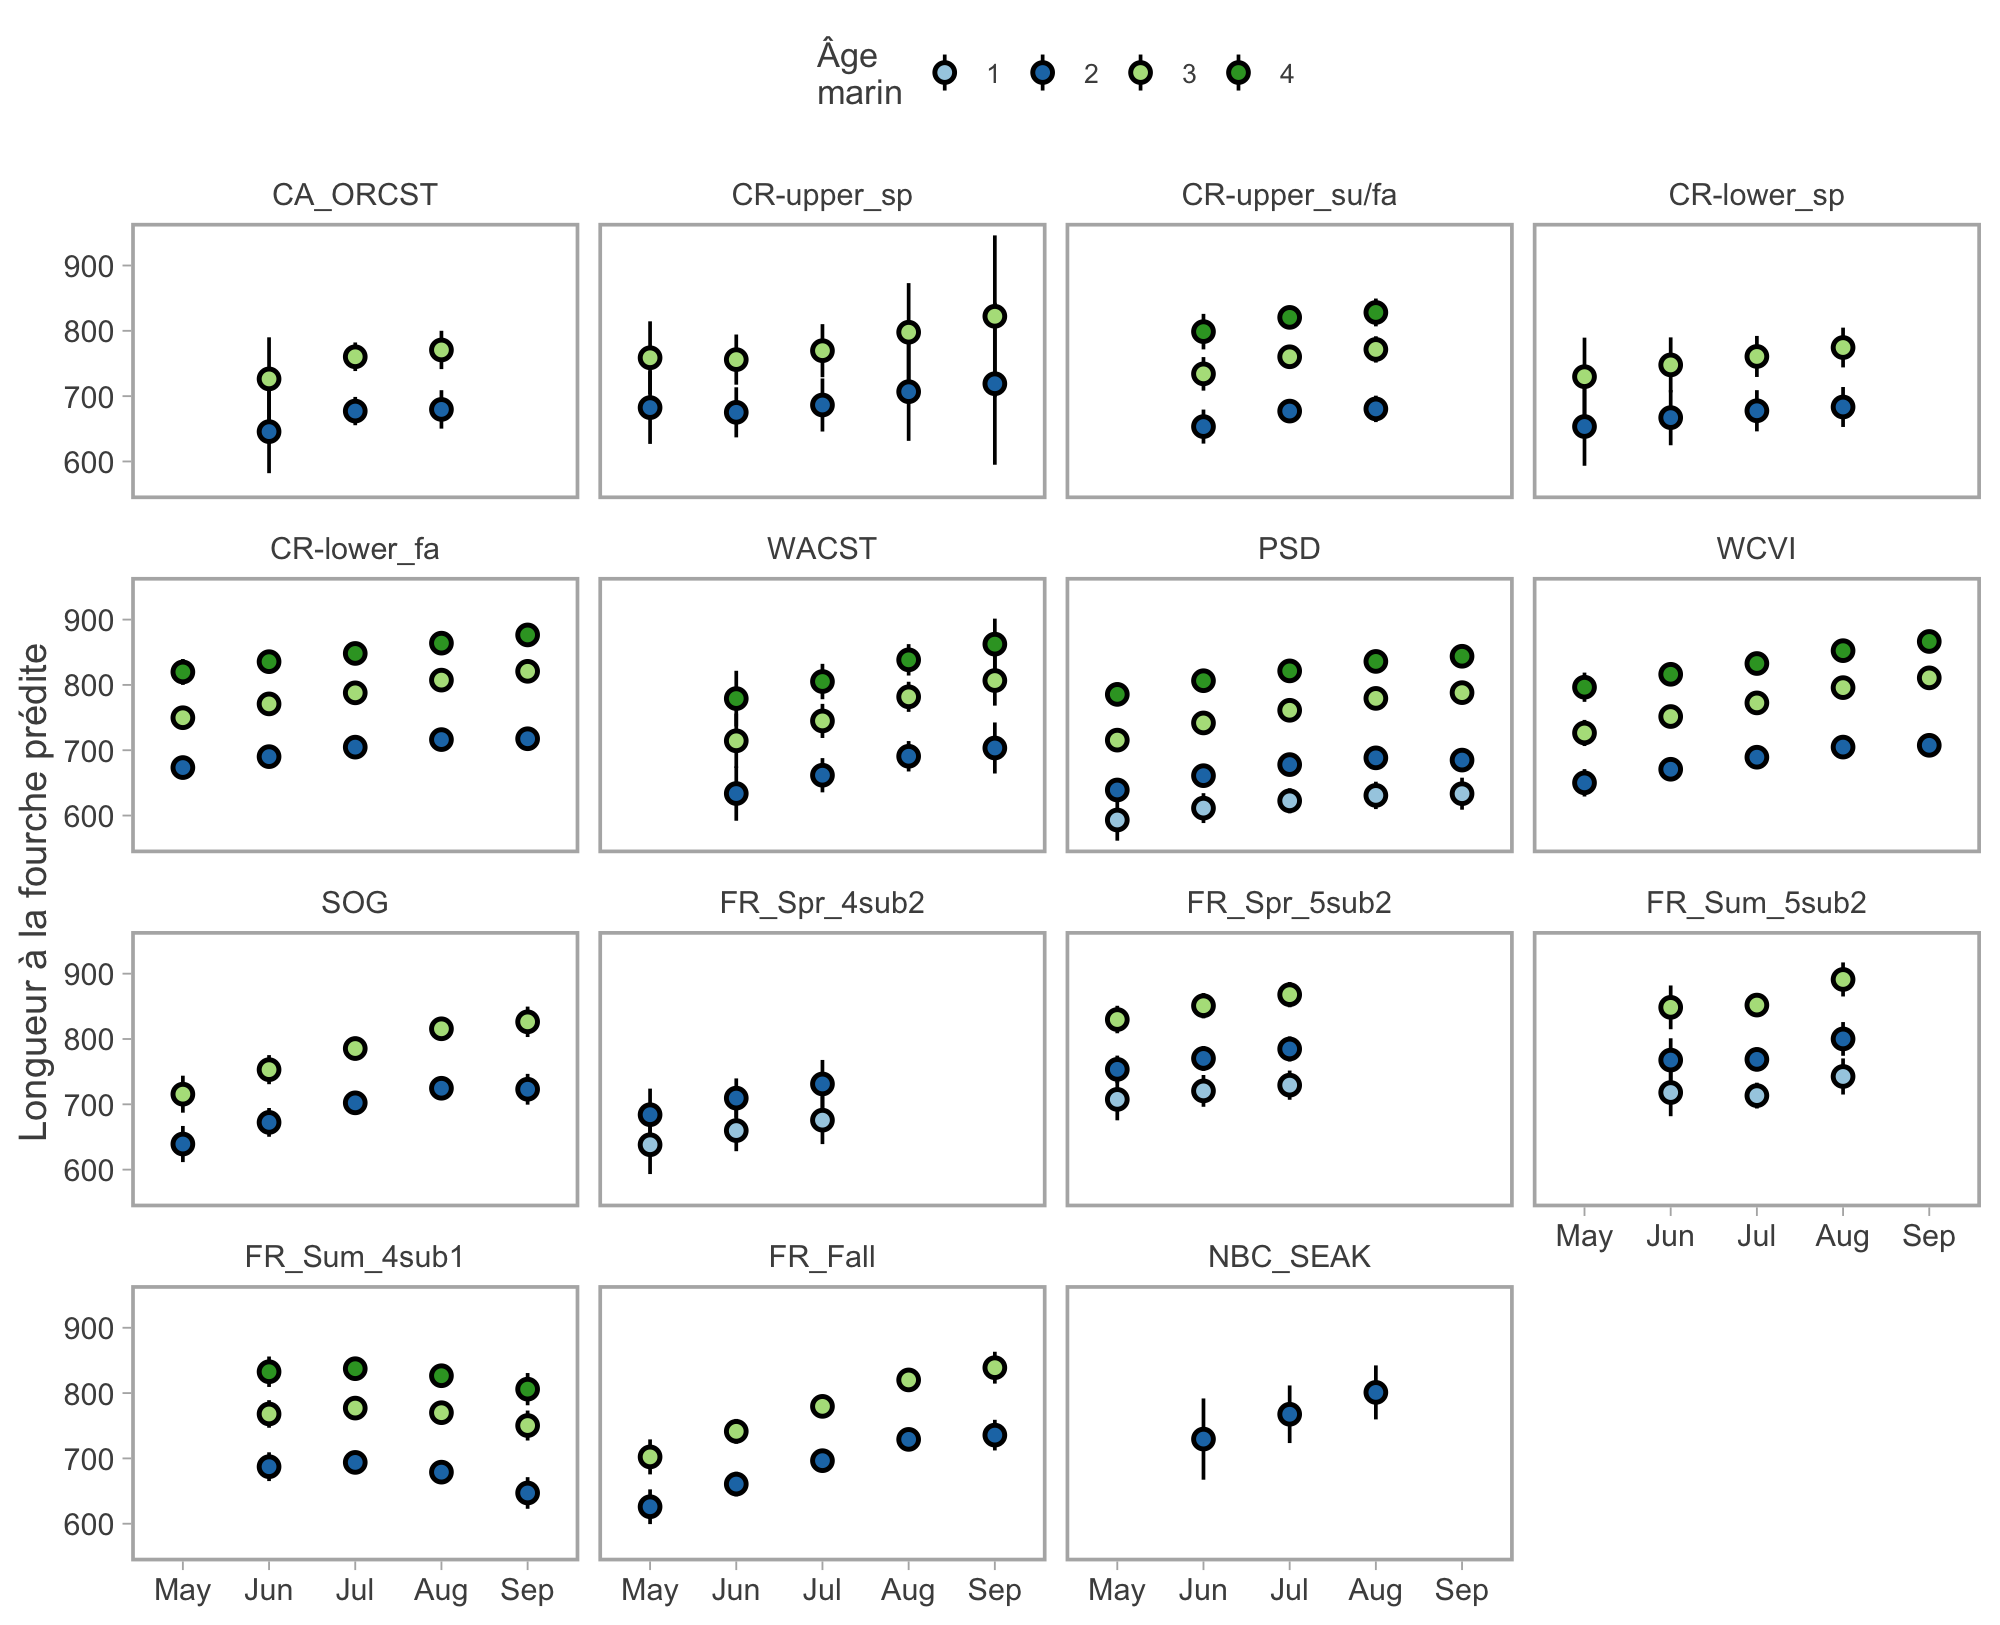
\includegraphics[width=5in]{figs/supp_figs/mean_pred_fishery.png}}{Figure \ref{fig:pred-size-at-age}}
    \caption{Taille selon l'âge prédite par le modèle. Les points représentent les moyennes et les moustaches les intervalles de confiance à 95\,\%. Les prédictions ne sont montrées que pour les mois et âges marins où au moins cinq individus du stock pertinent étaient disponibles pour paramétrer le modèle.}
    \label{fig:pred-size-at-age}
\end{figure}

\begin{figure}[htb]
    \centering
    \pdftooltip{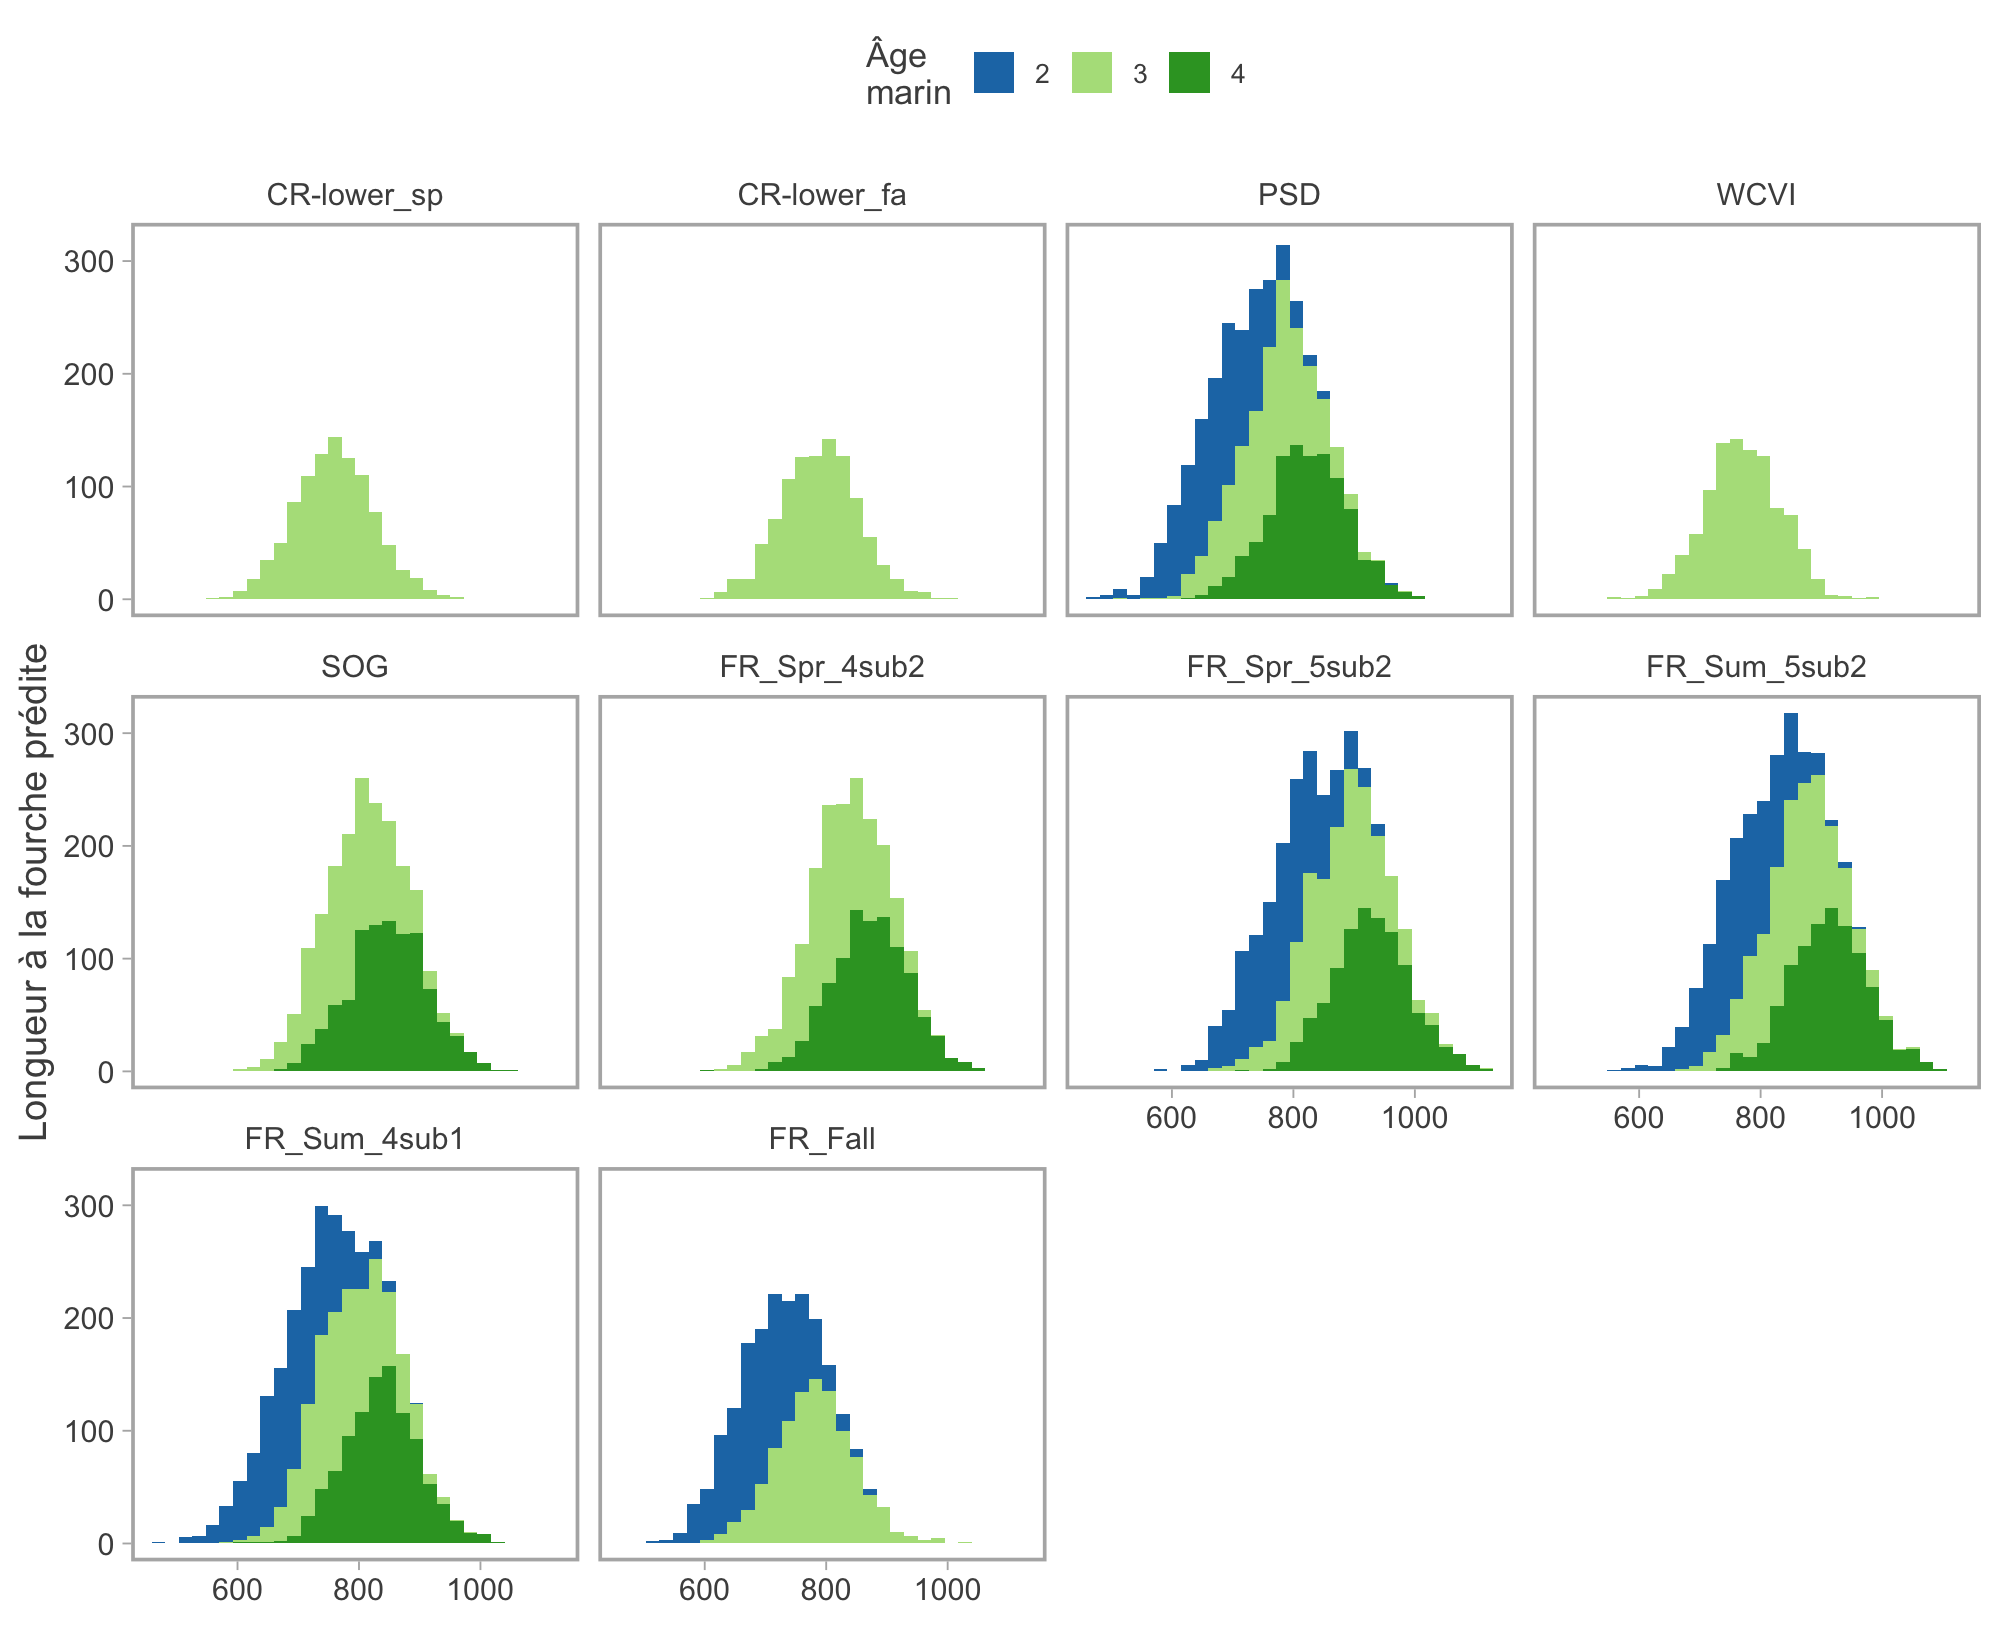
\includegraphics[width=5in]{figs/supp_figs/hist_pred_fishery.png}}{Figure \ref{fig:hist-size-at-age}}
    \caption{Distributions de taille selon l'âge prédites par le modèle pour juillet. Les distributions ont les mêmes moyennes que la Figure \ref{fig:pred-size-at-age}, mais incorporent la variabilité résiduelle autour de la moyenne. Seules les combinaisons d'âge et de stock observées dans les restes de proies des ERSN sont montrées.}
    \label{fig:hist-size-at-age}
\end{figure}

Nous avons utilisé le modèle ajusté pour générer une distribution postérieure de 1 000 échantillons de taille corporelle pour chaque combinaison de stock, d'âge marin et de mois observée dans les restes de proies des ERSN.

\appsection{Propagation de l'incertitude aux estimations de taille des restes de proies des ERSN}

Nous avons utilisé un processus en plusieurs étapes pour identifier un vecteur de probabilités qu'un échantillon donné de restes de proies des ERSN appartienne à une des quatre classes de taille $b'$. Premièrement, nous avons converti le vecteur de probabilités d'âge total $\boldsymbol{q_{a_t}}$ en un vecteur de probabilités d'âge marin $\boldsymbol{q_{a}}$, basé sur l'âge marin de l'échantillon lorsqu'une estimation était disponible ou basé sur l'histoire de vie dominante d'un stock autrement. Deuxièmement, pour chaque échantillon, nous avons tiré des distributions postérieures précédemment décrites d'estimations de taille corporelle spécifiques au stock, à l'âge marin et au mois proportionnellement à $\boldsymbol{q_{a}}$. En supposant que l'exemple précédemment décrit a été collecté en juin et appartenait à un individu Fraser Fall avec une probabilité de 50\,\% d'être âgé de 4 ans et une probabilité de 50\,\% d'être âgé de 5 ans, alors nous tirerions 500 échantillons de la distribution de taille Fraser Fall de juin âgé de 4 ans et 500 échantillons de la distribution de taille Fraser Fall de juin âgé de 5 ans (p. ex., Figures \ref{fig:pred-size-at-age}, \ref{fig:hist-size-at-age}). Troisièmement, nous avons converti chaque échantillon de taille en une classe de taille $b'$ et avons calculé la proportion des 1 000 échantillons appartenant à chaque classe, créant un vecteur de probabilités de classe de taille $q_{b'}$ pour chaque échantillon. 

Pour s'assurer que cette analyse était traitable, nous n'avons pas propagé l'incertitude d'assignation du stock. Au lieu de cela, nous avons utilisé la probabilité d'assignation de stock maximale pour chaque échantillon individuel pour générer $q_{b'}$. Nous croyons que cette supposition est peu susceptible d'impacter fortement nos résultats étant donné : des biais d'âge similaires entre les stocks, des distributions de taille selon l'âge largement chevauchantes entre les stocks (Figure \ref{fig:hist-size-at-age}), les échantillons de proies avec une probabilité d'assignation inférieure à 60\,\% ont été exclus, et qu'environ 90\,\% des échantillons inclus avaient une probabilité d'assignation supérieure à 80\,\%.